\section{Vorbereitung der 3D Modelle in Blender}
Einige 3D Modelle haben durch die umliegende Vegetation unvollständige oder mit der Vegetation verschmolzene Meshes. In der Projektarbeit des Wintersemesters 2020/21 wird das Problem näher beschrieben \cite*{kusch2021}.

\subsection{Lückenhafte Wände füllen}
Das Gebäude 2 des Lyautey Geländes hat eine Haushälfte, die mit einem Baum verschmolzen ist und es fehlt daher ein Teil der Wand. Da das Gebäude symmetrisch und die gespiegelte Seite fehlerfrei ist, wird ein Teil dieser Wand als Lückenfüller eingesetzt. Im folgenden wird die Nachbearbeitung an diesem Modell beschrieben.

\begin{figure}[ht]
    \centering
    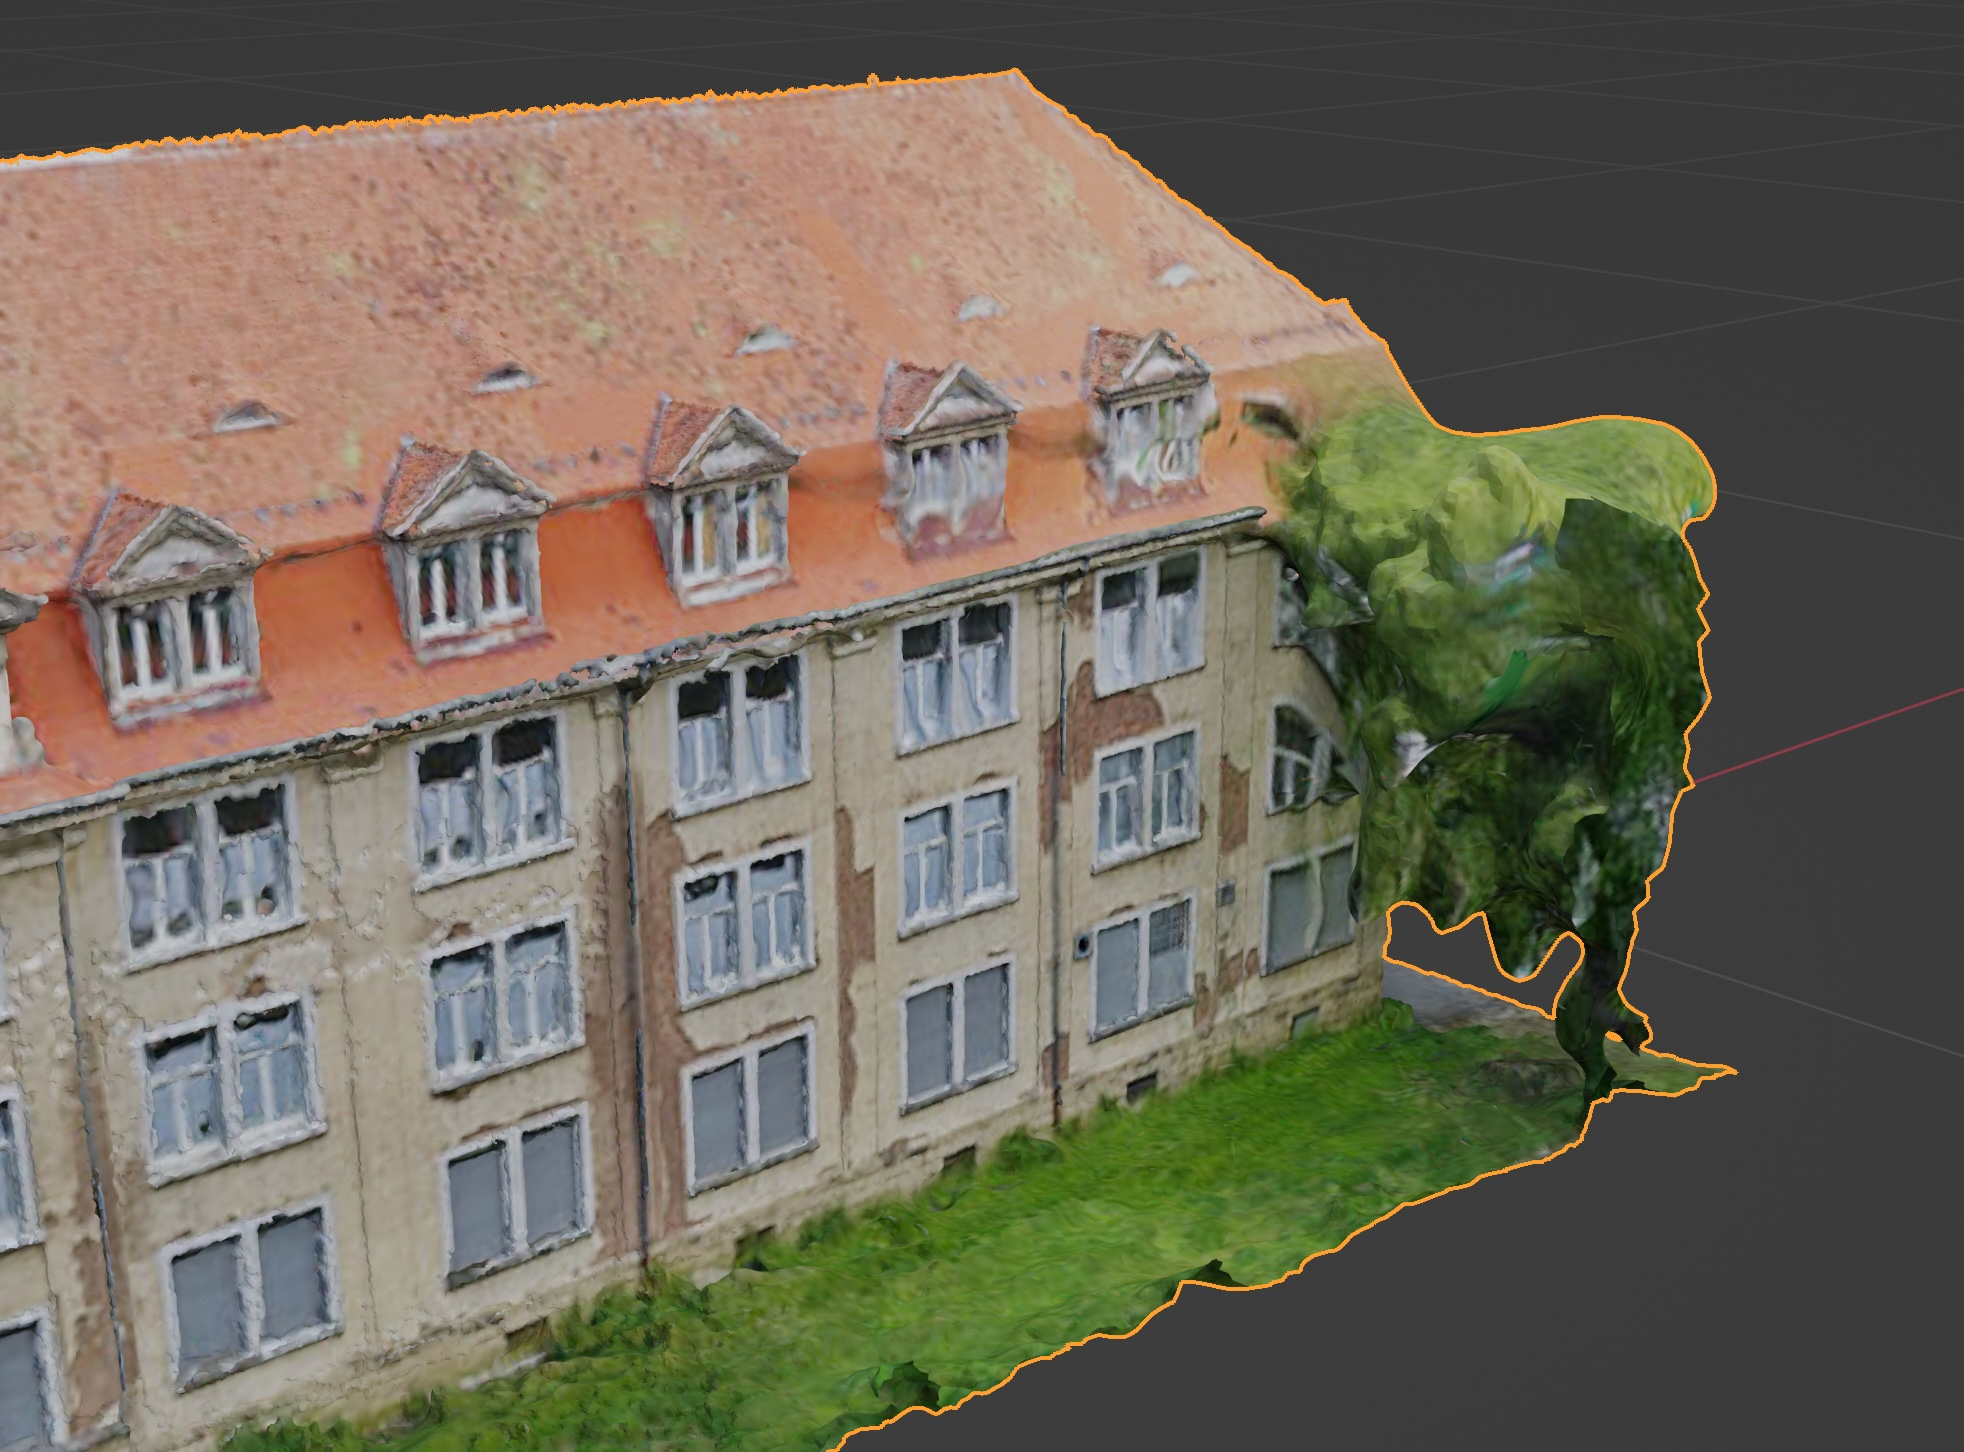
\includegraphics[width=0.5\textwidth]{img/vorbereitungen_blender_modelle/g2_verschmolzen.jpg}
    \caption{Ein Baum behinderte bei den Aufnahmen die Sicht auf die Wand, sodass diese mit dem Baum verschmolzen ist.}
    \label{fig:g2_verschmolzen}
\end{figure}

Zunächst wird das Modell kopiert. Anschließend werden die fehlerhaften Polygone im \textit{Edit-Mode} ausgewählt und gelöscht. Beim kopierten Modell werden alle Polygone gelöscht, bis auf die Wand, die eingesetzt werden soll. Diese wird mit dem \textit{Mirror-Modifier} gespiegelt. Das gespiegelte Modell wird an die Position der fehlerhaften Wand gesetzt und die beiden Modelle werden mit \textit{STRG + J} als ein Modell zusammengefügt. Die Lücke zwischen den beiden Modellen wird anschließend händisch mit neuer Geometrie gefüllt. Dieser Prozess ist sehr zeitaufwendig, da je nach Polygonanzahl viele Kanten einzeln ausgewählt werden müssen. Daher wird zunächst ein \textit{Decimate-Modifier} benutzt, um die Anzahl an Polygone zu reduzieren. Bei diesem Gebäude wird eine Reduzierung um 70\% vorgenommen, sodass sich die gesamte Anzahl an Polygonen von über 2.5 Millionen auf ca 750.000 Polygone verringert, ohne einen starken Verlust im Detailgrad festzustellen.

\begin{figure}[hbt!]
    \centering
    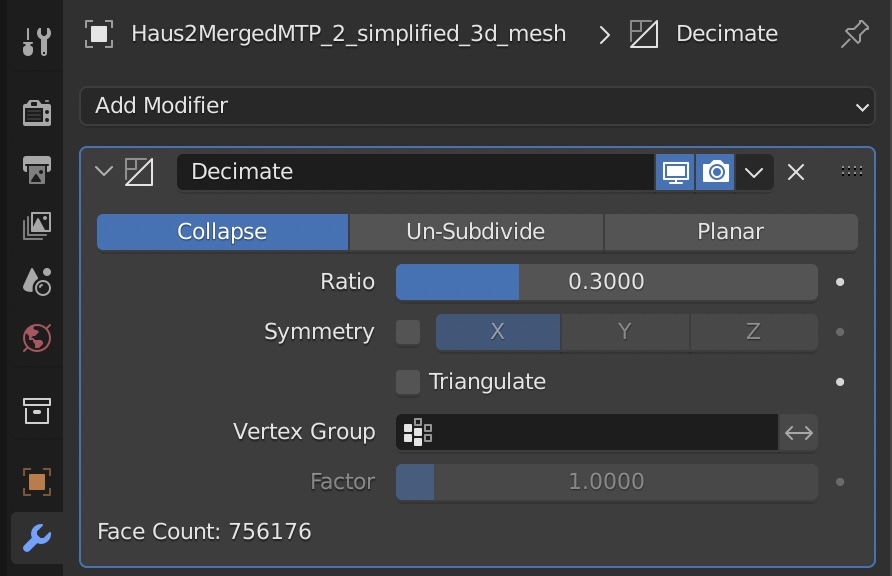
\includegraphics[width=0.5\textwidth]{img/vorbereitungen_blender_modelle/blender_decimate.jpg}
    \caption{Der Decimate-Modifier reduziert die Anzahl an Polygonen. Ein Wert von 0.3 beduetet, dass die Polygonenanzahl 30\% der ursprünglichen Polygonanzahl entspricht.}
    \label{fig:blender_decimate_modifier}
\end{figure}

Um die Lücken zu schließen werden benachbarte Kanten im \textit{Edit-Mode} ausgewählt und mit der \textit{F-Taste} mit neuen Flächen aufgefüllt. An einigen Stellen sind kleine Polygone vorhanden, bei dem dieser Prozess erschwert wird. Diese werden gelöscht und mit größeren Flächen ersetzt.  

\begin{figure}[hbt!]
    \centering
    \subfloat[][]{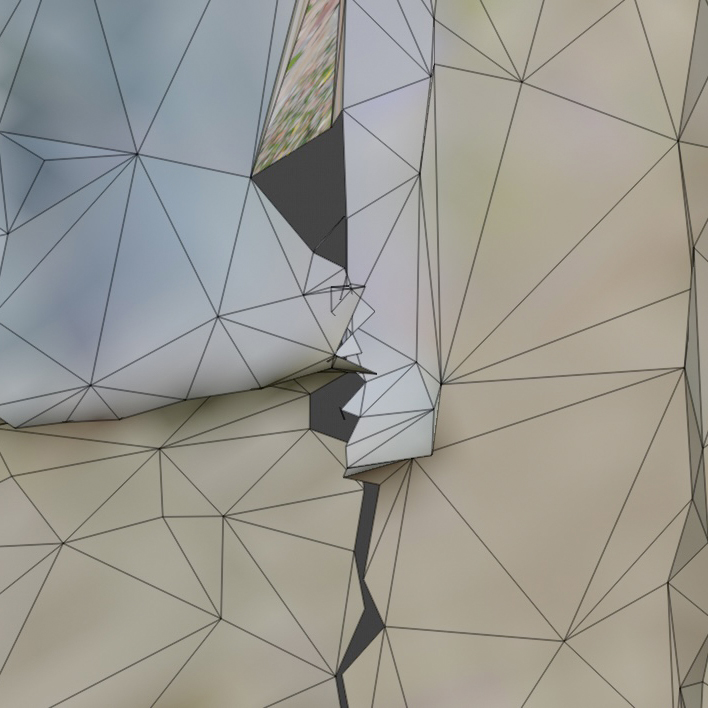
\includegraphics[width=0.4\linewidth]{img/vorbereitungen_blender_modelle/kleine_polygone_entfernen_1.jpg}}%
    \qquad
    \subfloat[][]{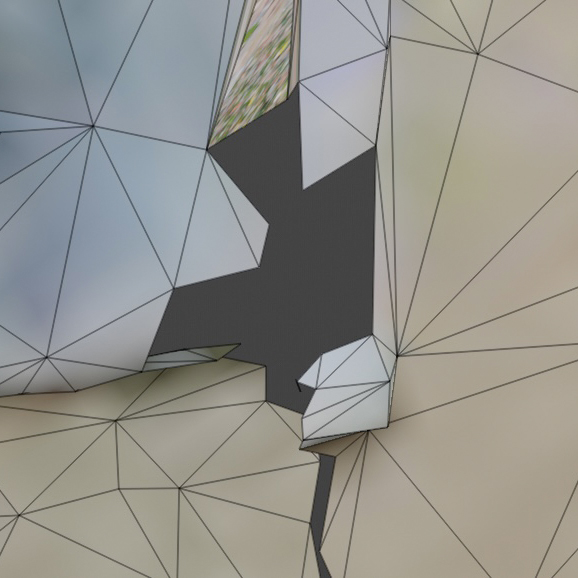
\includegraphics[width=0.4\linewidth]{img/vorbereitungen_blender_modelle/kleine_polygone_entfernen_2.jpg}}%
    \caption{Kleine Polygone erschweren das Markieren von Kanten (a). Das entstandene Loch wird mit größeren Flächen gefüllt (b).}%
    \label{fig:blender_kleine_polygone}
\end{figure}

\begin{figure}[hbt!]
    \centering
    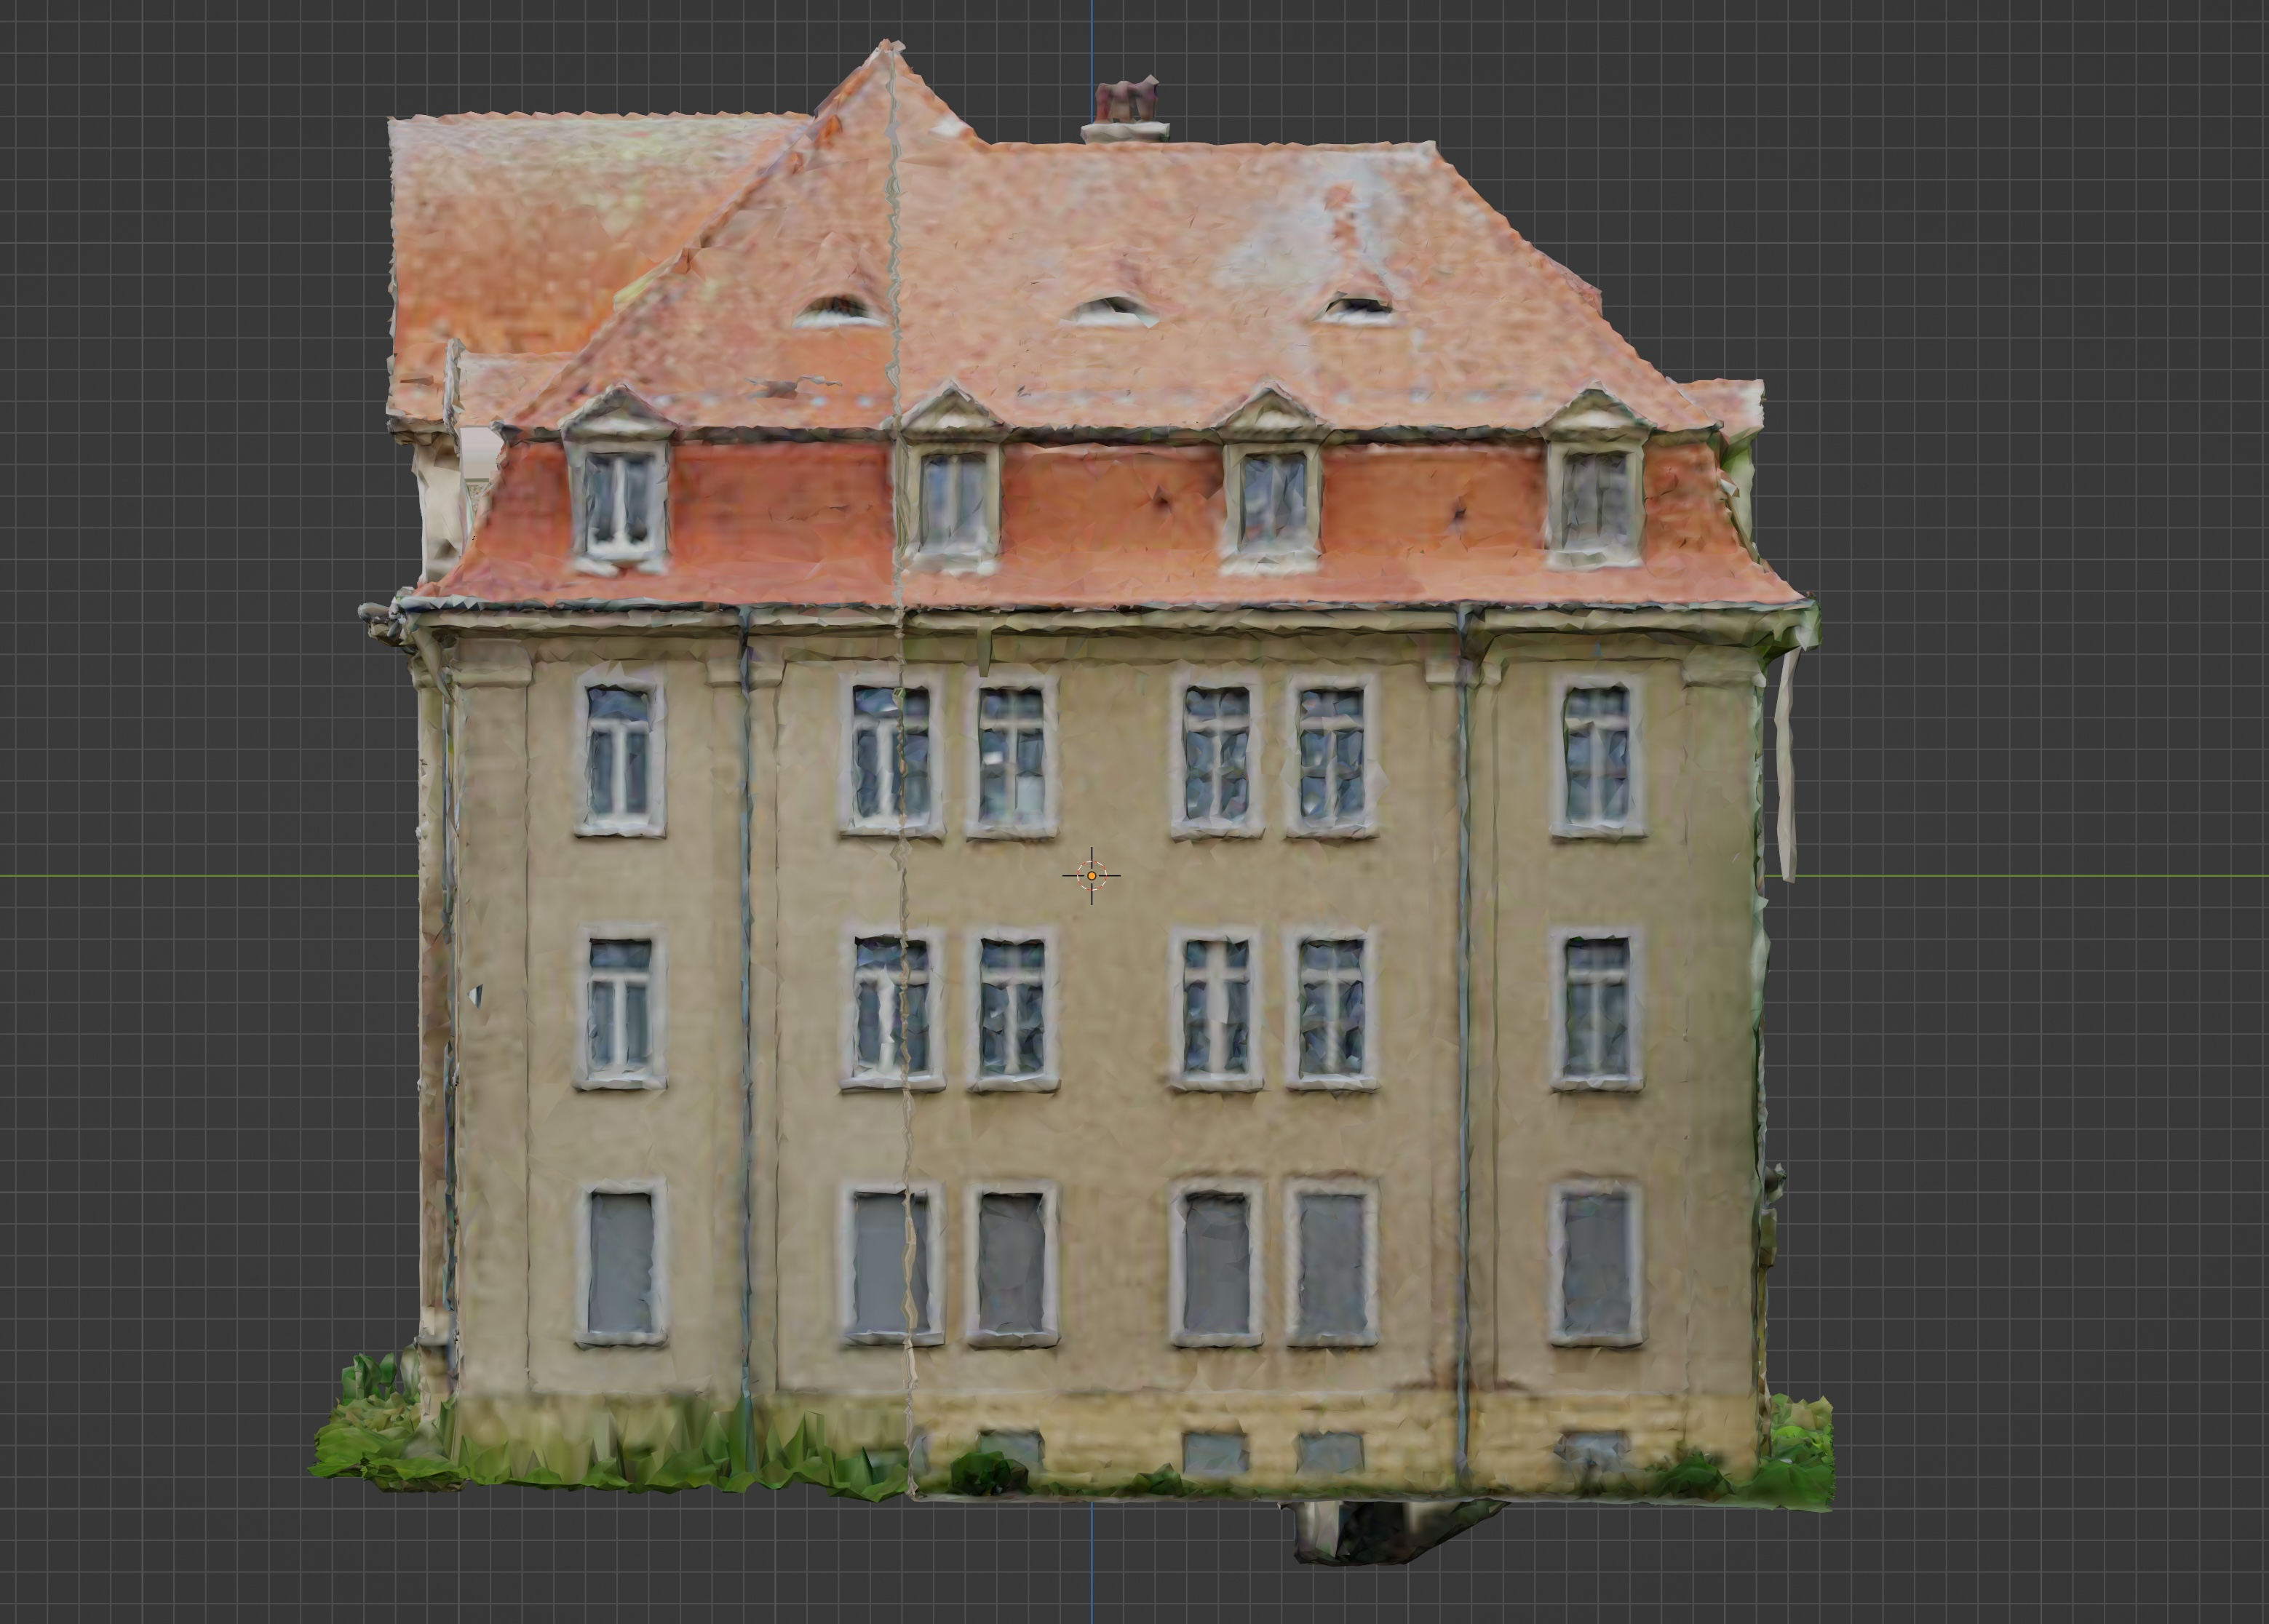
\includegraphics[width=0.5\textwidth]{img/vorbereitungen_blender_modelle/g2_naht.jpg}
    \caption{Das zusammengesetzte Gebäude.}
    \label{fig:blender_naht}
\end{figure}

Ist der Füllprozess abgeschlossen, ist die Naht dennoch erkennbar (siehe Abbildung \ref*{fig:blender_naht}), da die Textur auf den neuen Polygonen verzerrt wird. Aufgrunddessen werden im letzten Schritt im UV-Editing Tab die UV-Koordinaten der neuen Polygone neu vergeben, sodass die Texturen den umliegenden Flächen entsprechen. Hierfür werden die neuen Polygone im \textit{Edit-Mode} markiert. Im \textit{UV-Editor} werden mit dem Befehl \textit{U + Unwrap} die markierten Polygone bestmöglich auf die 2D Textur gelegt.\footnote{https://docs.blender.org/manual/en/latest/modeling/meshes/editing/uv.html, zuletzt augerufen am 29.05.2022} Die Polygone werden auf der Textur so skaliert, bewegt und rotiert, dass sie eine ähnliche Textur wie die umliegenden Flächen besitzen. Zur Hilfe werden die umliegenden Flächen markiert und deren UV-Koordinaten auf der Textur verglichen. So wird sichergestellt, dass die Farbunterschiede an den Kanten nicht zu stark abweichen. Das fertige Modell ist im Vorher-Nachher-Vergleich in Abbildung \ref*{fig:blender_vergleich} zu sehen. 

\begin{figure}[hbt!]
    \centering
    \subfloat[][]{\includegraphics[width=0.4\linewidth]{img/vorbereitungen_blender_modelle/polygone_markieren.jpg}}%
    \qquad
    \subfloat[][]{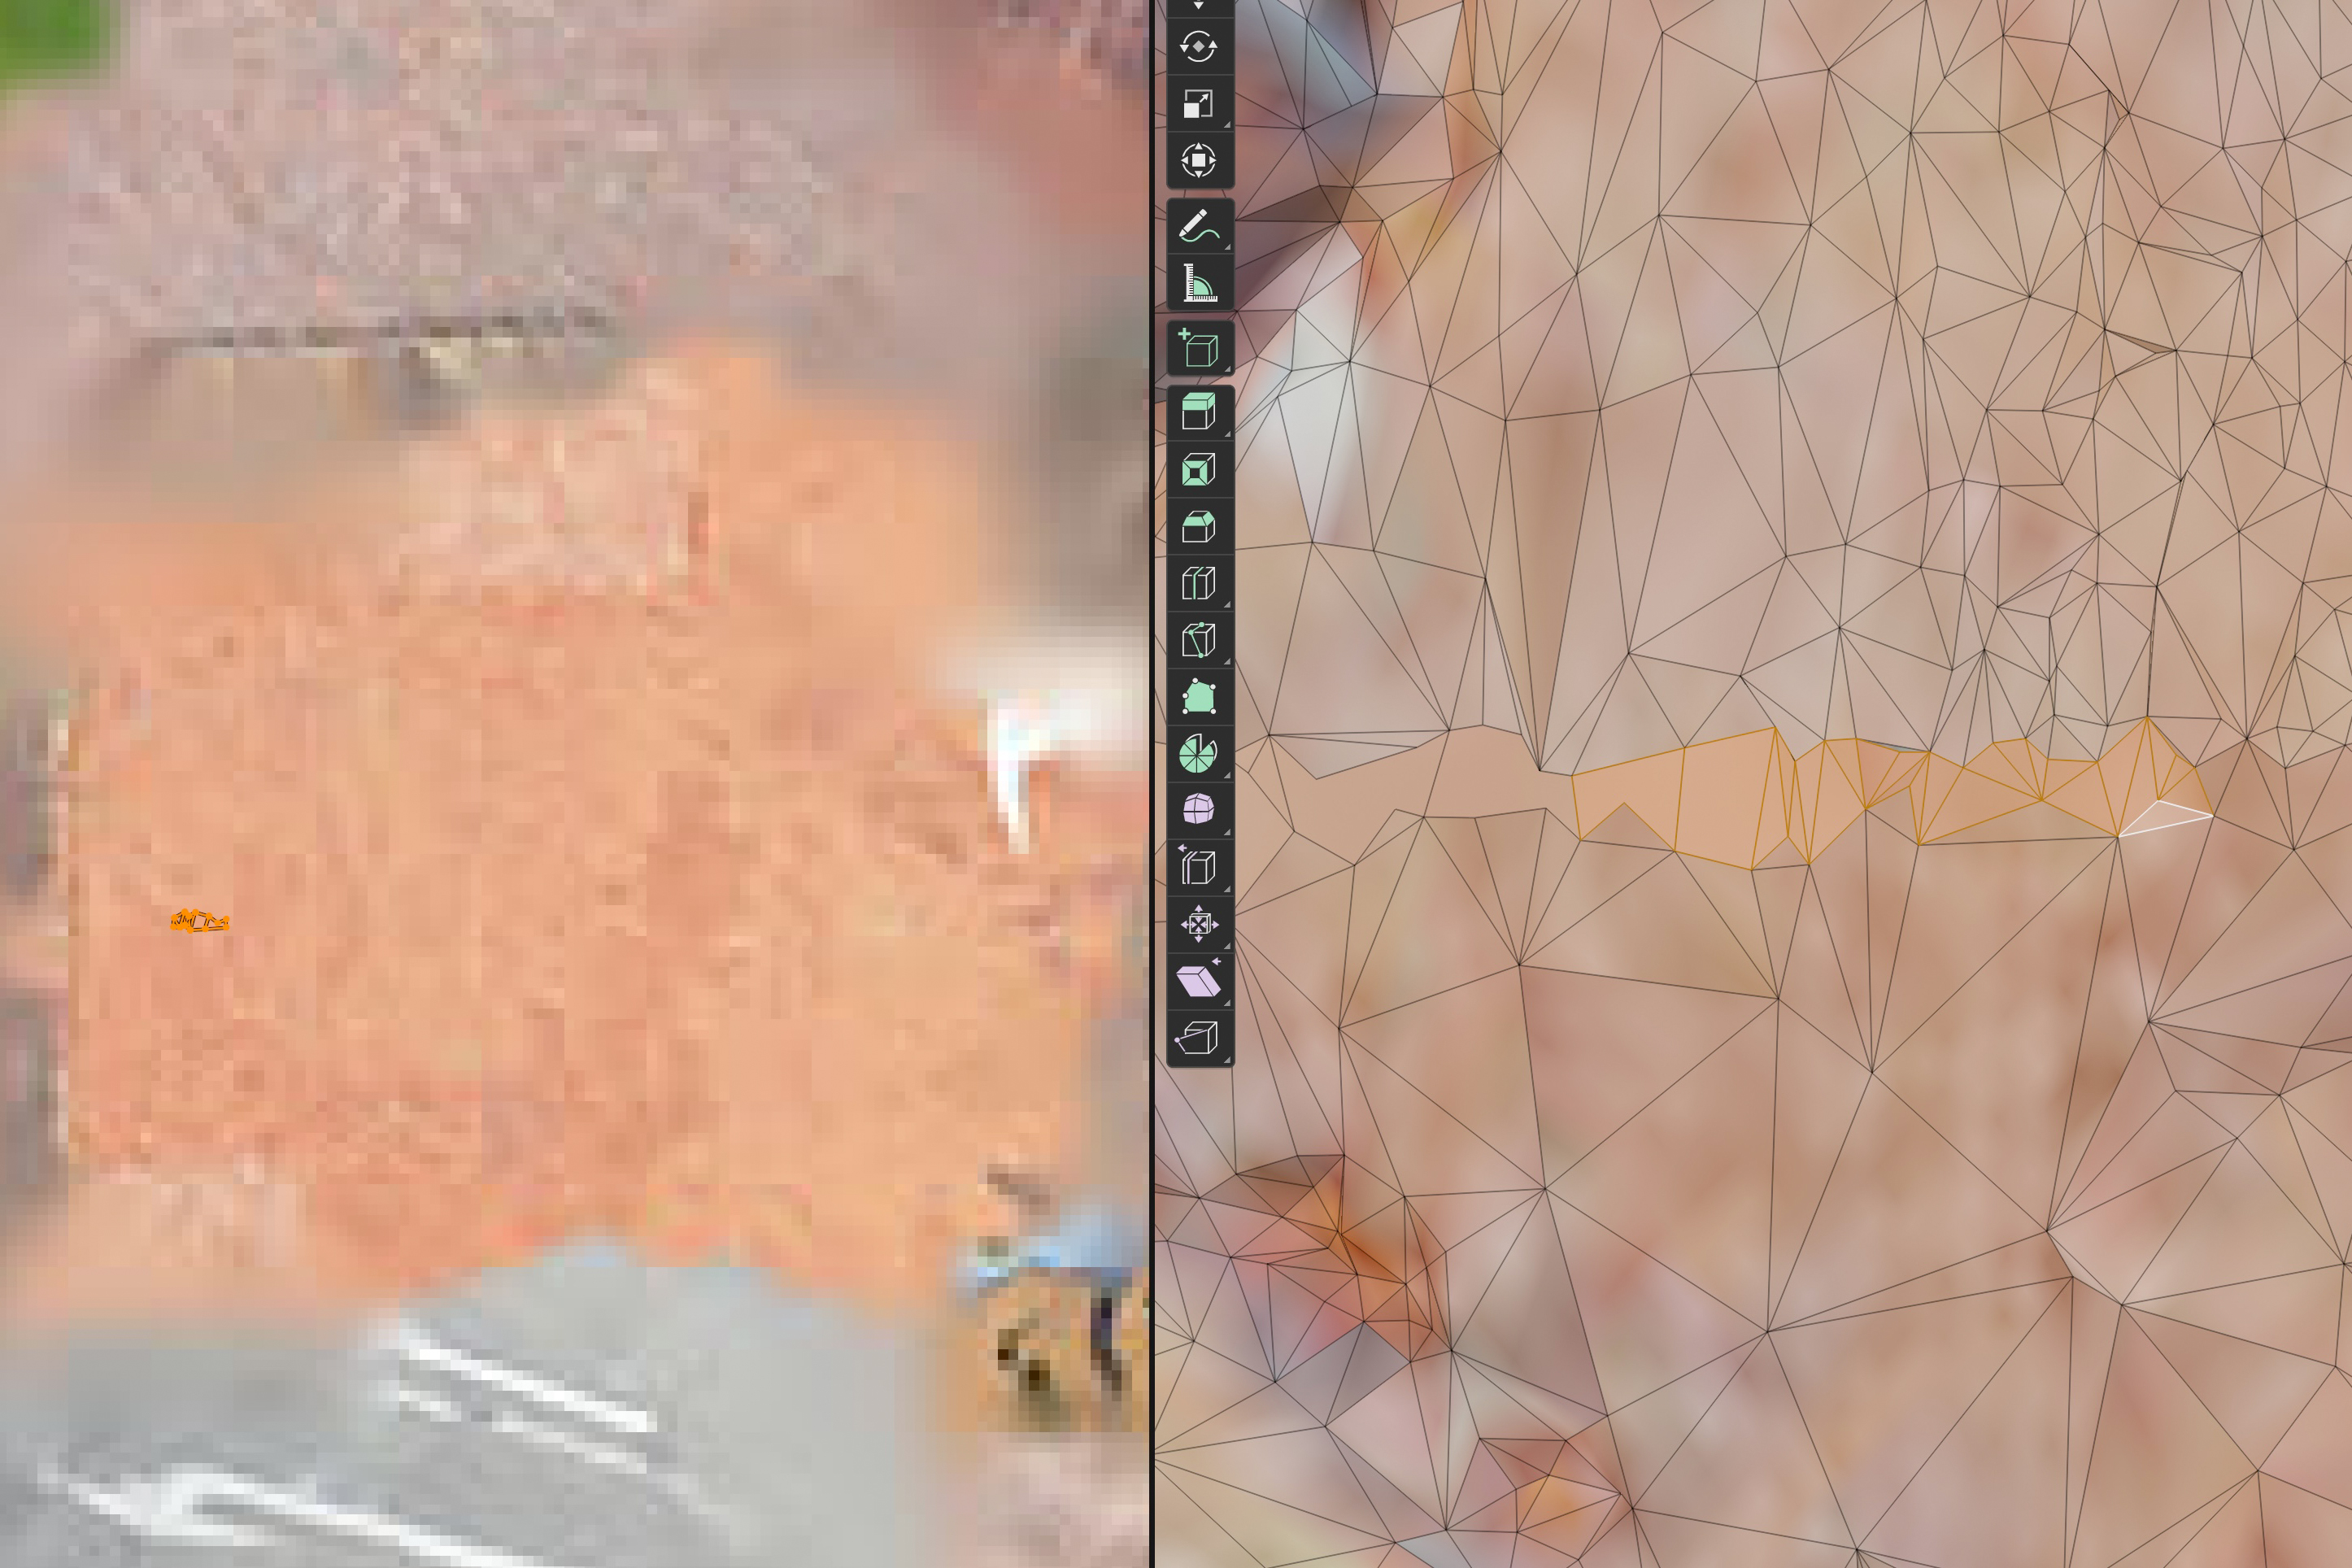
\includegraphics[width=0.4\linewidth]{img/vorbereitungen_blender_modelle/polygone_textur.jpg}}%
    \caption{Die Polygone werden markiert(a), unwrapped und anschließend auf eine geeignete Fläche auf der Textur gelegt(b).}%
    \label{fig:blender_uv_editing}
\end{figure}

\begin{figure}[hbt!]
    \centering
    \subfloat[][]{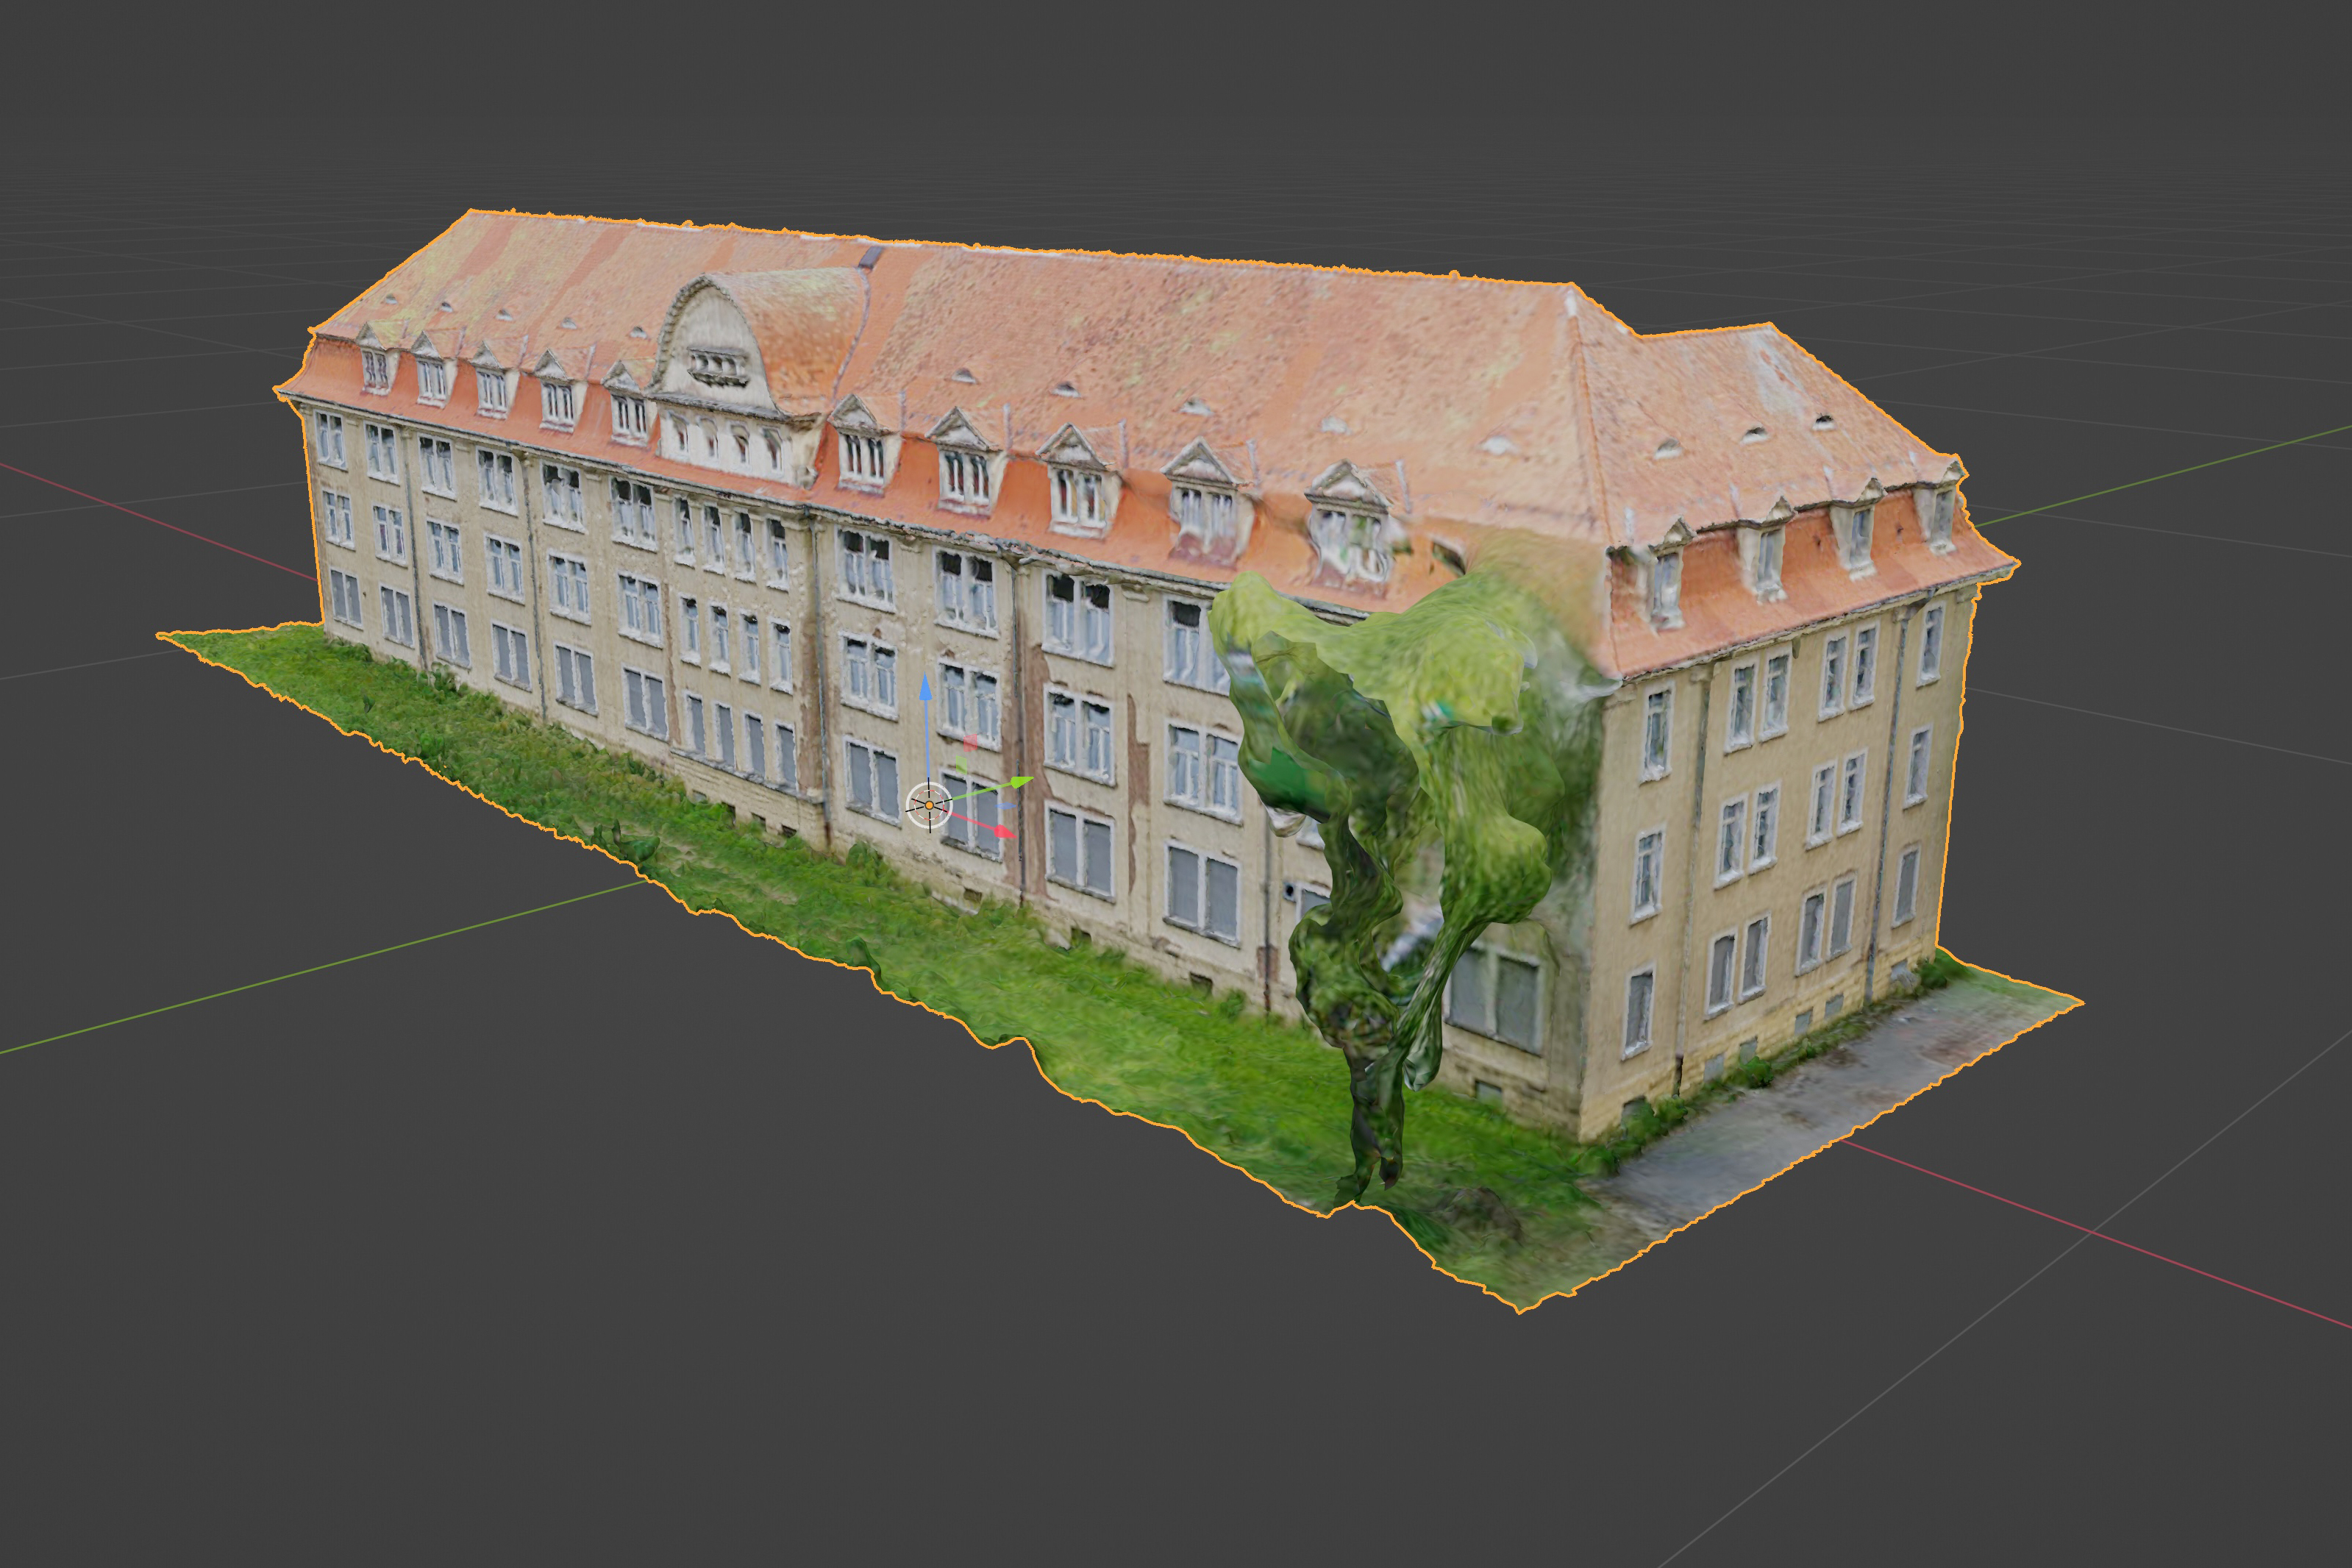
\includegraphics[width=0.4\linewidth]{img/vorbereitungen_blender_modelle/blender_vorher.jpg}}%
    \qquad
    \subfloat[][]{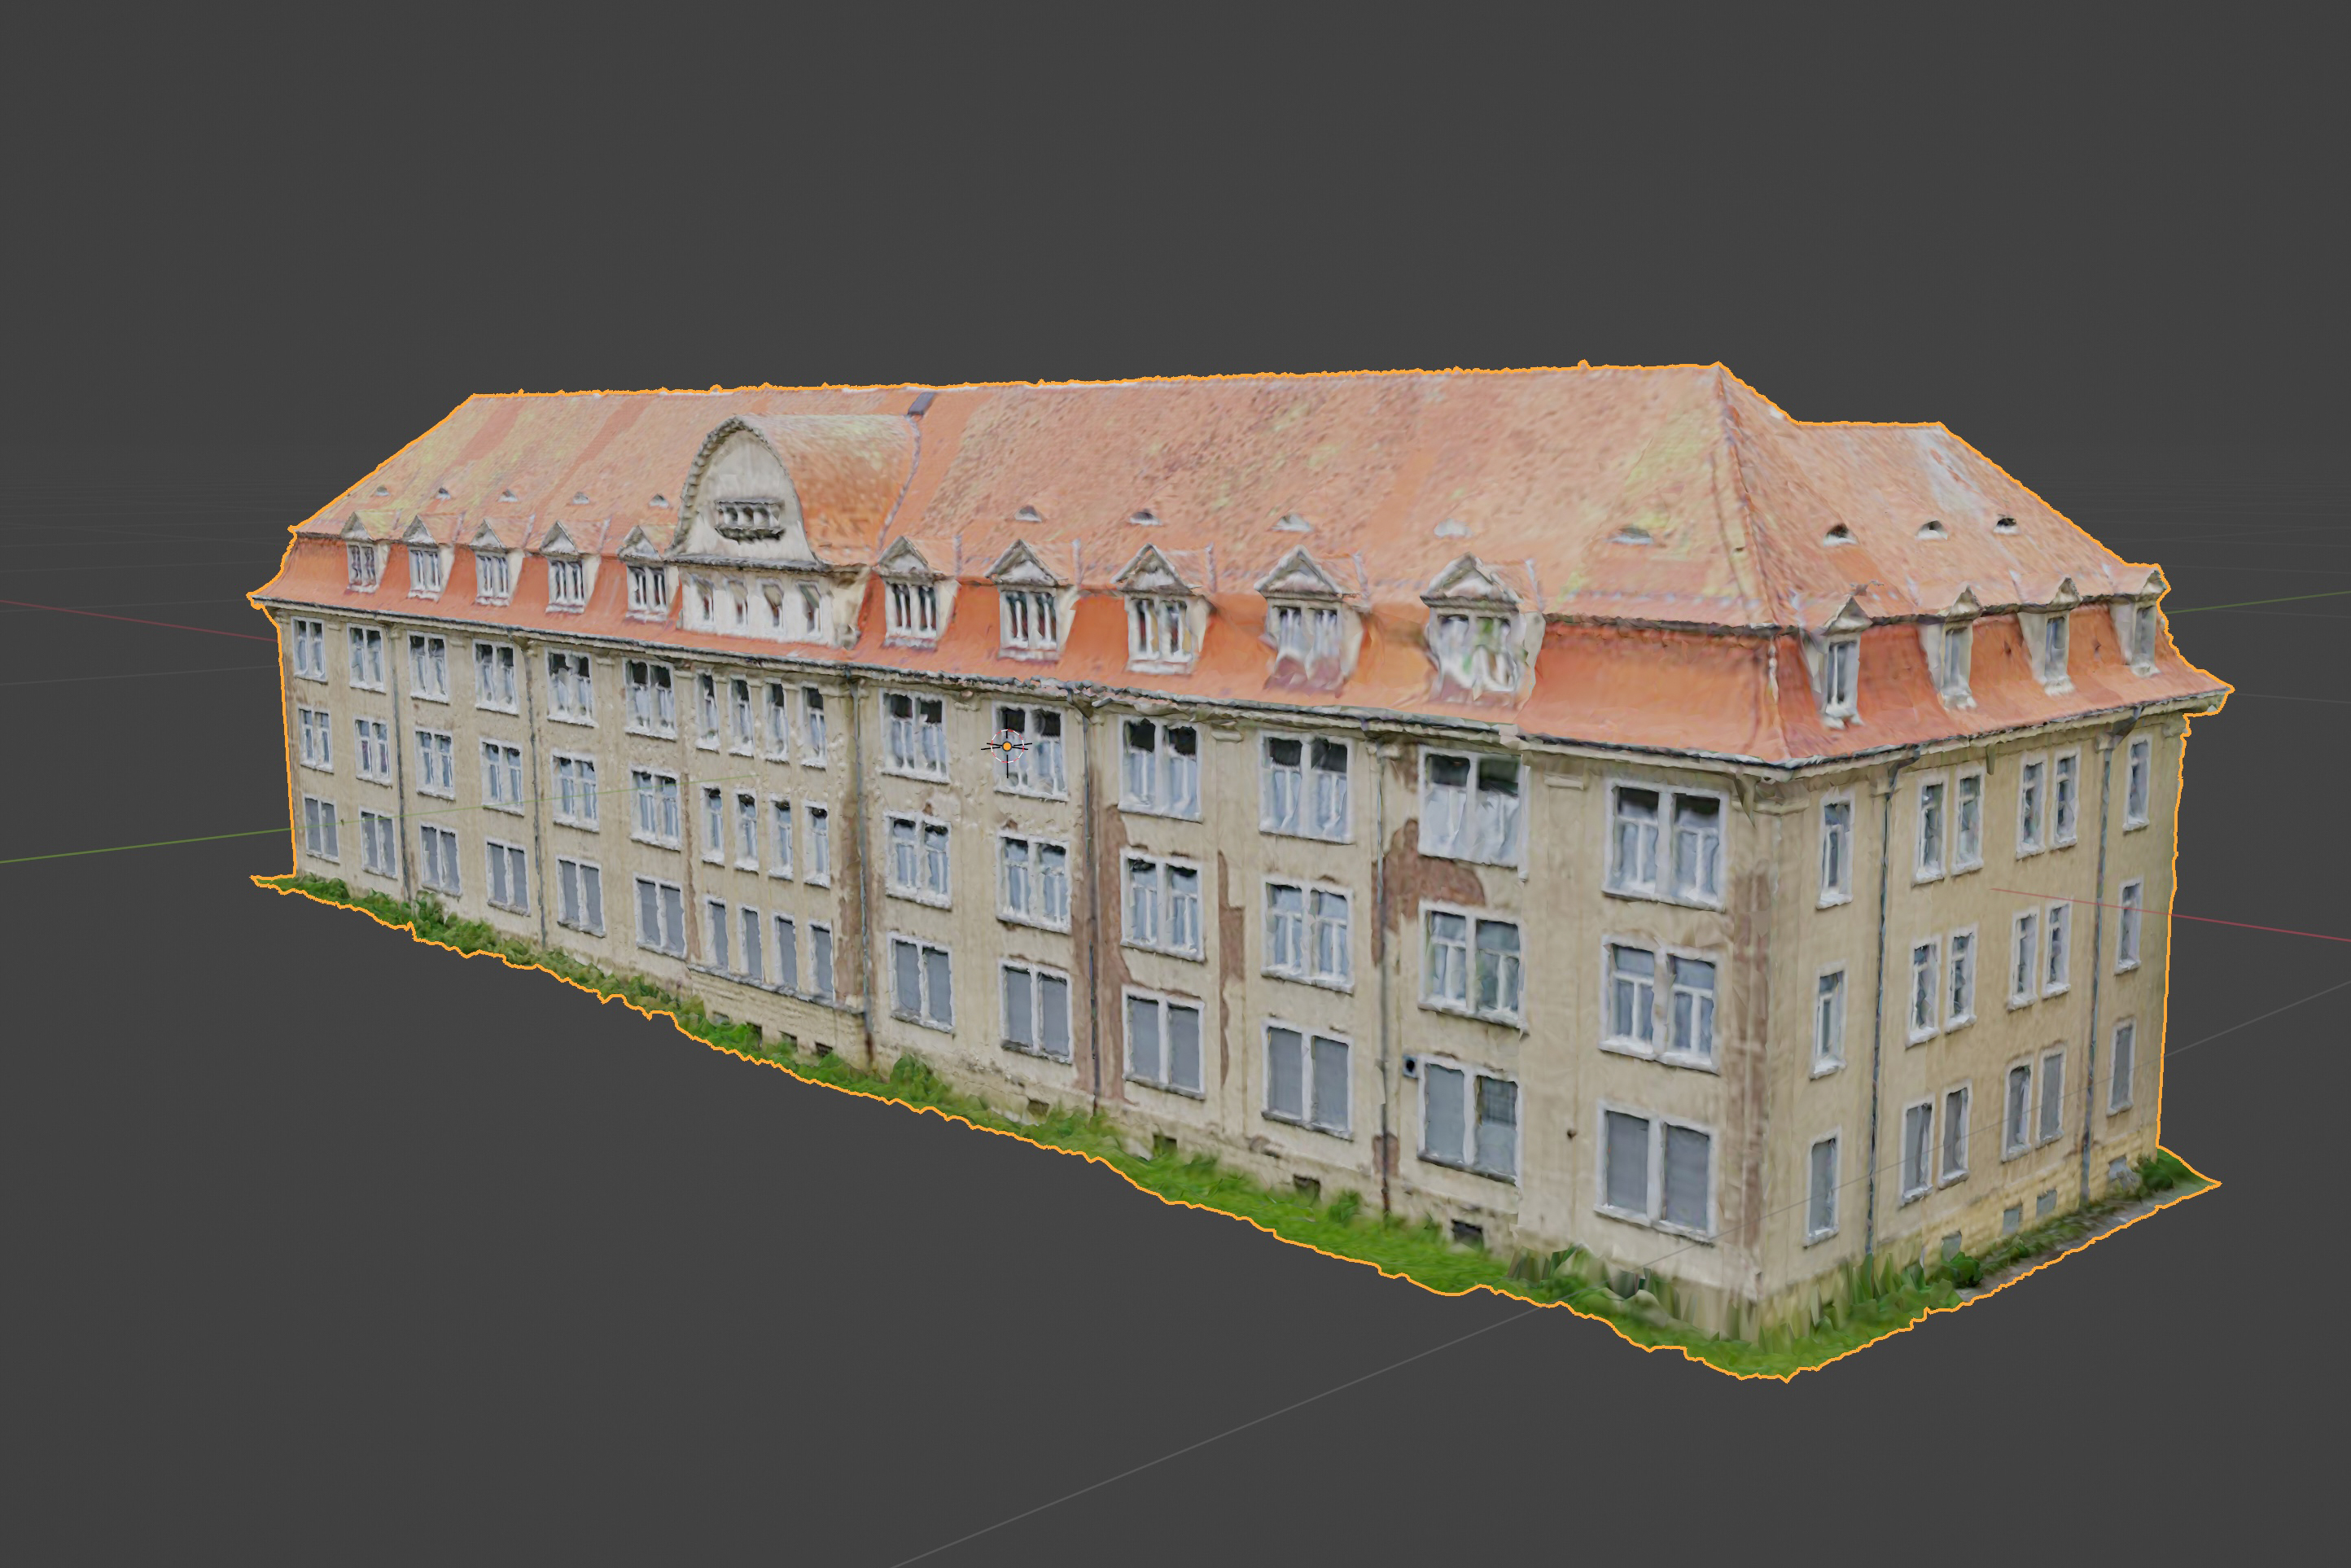
\includegraphics[width=0.4\linewidth]{img/vorbereitungen_blender_modelle/blender_nachher.jpg}}%
    \caption{Das Mannschaftsgebäude vor(a) und nach der Bearbeitung(b).}%
    \label{fig:blender_vergleich}
\end{figure}

\subsection{Export und Import}
Damit Unity die 3D Modelle korrekt darstellen kann, werden Anpassungen in Blender vorgenommen:

\begin{itemize}
    \item Vor dem Export werden Texturen in einem Ordner gespeichert. In Blender muss dafür die Option unter \textit{File>External Data>Automatically Pack Resources} ausgeschaltet sein. Anschließend wird mit \textit{File>External Data>Unpack Resources} ein Ordner im Projekt mit den Namen \textit{textures} erstellt, in dem sich die Texturen des Projekts befinden. Nun kann Unity die fehlenden Materials und Texturen im Projekt-Ordner finden,
    \item Unity kann die Texturen nur anwenden, wenn die Textur direkt im \textit{Shader Node} als \textit{Base Color} verbunden ist. Dazwischen befindliche Knoten funktionieren nur in Blender und müssen entfernt werden,
    \item die in Blender genutzten \textit{Modifier}\footnote{https://docs.blender.org/manual/en/latest/modeling/modifiers/index.html} werden angewendet,
    \item damit die Textur korrekt dargestellt werden, werden die Richtungen der \textit{Normalen}\footnote{https://docs.blender.org/manual/en/latest/modeling/meshes/editing/mesh/normals.html?highlight=normals} überprüft, ob diese in die richtige Richtung zeigen. Die Normalen müssen zur korrekten Darstellung nach außen zeigen. In Blender können die Normalen im \textit{Edit Mode} im Viewport Overlay angezeigt und unter \textit{Mesh>Normals} angepasst werden,
    \item Blender und Unity haben unterschiedliche Koordinatensysteme. In Blender zeigt die Z-Achse nach oben und die Y-Achse in die Tiefe, während in Unity die Y-Achse nach oben und die Z-Achse in die Tiefe zeigt. Damit die Modelle aus Blender mit der korrekten Orientierung dargestellt werden, wird das Modell in Blender um -90° gedreht. Mit \textit{STRG + A} und \textit{Rotation} wird die Rotation eingebettet,
    \item beim Export wird das Export-Format \textit{.fbx} benötigt.
\end{itemize}

Jetzt wird das 3D Modell als \textit{.fbx} Datei in Unity importiert. Im \textit{Inspector}-Fenster der \textit{.fbx} Datei werden unter Materials mit \textit{Exctract Materials} Materials in Unity generiert, die die Texturen beinhalten. Der Texturen-Ordner muss im gleichen Ordner liegen. Werden die Texturen nicht gefunden, so können diese händisch in das Projekt eingefügt werden. Um die Texturen den von Unity generierten Materials zu geben, wird im \textit{Inspector} die Textur in das Feld neben \textit{Albedo} eingefügt werden.